\documentclass[12pt, titlepage]{article}

\usepackage{fullpage}
\usepackage[round]{natbib}
\usepackage{multirow}
\usepackage{booktabs}
\usepackage{tabularx}
\usepackage{graphicx}
\usepackage{float}
\usepackage{hyperref}
\hypersetup{
    colorlinks,
    citecolor=blue,
    filecolor=black,
    linkcolor=red,
    urlcolor=blue
}
%% Comments

\usepackage{color}

\newif\ifcomments\commentstrue %displays comments
%\newif\ifcomments\commentsfalse %so that comments do not display

\ifcomments
\newcommand{\authornote}[3]{\textcolor{#1}{[#3 ---#2]}}
\newcommand{\todo}[1]{\textcolor{red}{[TODO: #1]}}
\else
\newcommand{\authornote}[3]{}
\newcommand{\todo}[1]{}
\fi

\newcommand{\wss}[1]{\authornote{blue}{SS}{#1}} 
\newcommand{\plt}[1]{\authornote{magenta}{TPLT}{#1}} %For explanation of the template
\newcommand{\an}[1]{\authornote{cyan}{Author}{#1}}

%% Common Parts

\newcommand{\progname}{Sayyara Automotive Matcher} % PUT YOUR PROGRAM NAME HERE
\newcommand{\authname}{Team 27, Kappastone
\\ Tevis Doe, doet
\\ Caitlin Bridel, bridelc
\\ Gilbert Cherrie, cherrieg
\\ Rachel Johnson, johnsr12
\\ Harkeerat Kanwal, kanwalh
\\ Himanshu Aggarwal, aggarwah} % AUTHOR NAMES                  

\usepackage{hyperref}
    \hypersetup{colorlinks=true, linkcolor=blue, citecolor=blue, filecolor=blue,
                urlcolor=blue, unicode=false}
    \urlstyle{same}
                                


\newcounter{acnum}
\newcommand{\actheacnum}{AC\theacnum}
\newcommand{\acref}[1]{AC\ref{#1}}

\newcounter{ucnum}
\newcommand{\uctheucnum}{UC\theucnum}
\newcommand{\uref}[1]{UC\ref{#1}}

\newcounter{mnum}
\newcommand{\mthemnum}{M\themnum}
\newcommand{\mref}[1]{M\ref{#1}}

\begin{document}

\title{Module Guide for \progname{}} 
\author{\authname}
\date{\today}

\maketitle

\pagenumbering{roman}

\section{Revision History}

\begin{tabularx}{\textwidth}{p{4cm}p{2cm}X}
\toprule {\bf Date} & {\bf Version} & {\bf Notes}\\
\midrule
January 18th, 2023 & 0.0 & Rev 0\\
\bottomrule
\end{tabularx}

\newpage

\section{Reference Material}

This section records information for easy reference.

\subsection{Abbreviations and Acronyms}

\renewcommand{\arraystretch}{1.2}
\begin{tabular}{l l} 
  \toprule		
  \textbf{symbol} & \textbf{description}\\
  \midrule 
  AC & Anticipated Change\\
  DAG & Directed Acyclic Graph \\
  FR & Functional Requirement\\
  M & Module \\
  MG & Module Guide \\
  OS & Operating System \\
  PWA & Progressive Web Application \\
  \progname & PWA for maintenance appointment scheduling for vehicle owners\\
  SRS & Software Requirements Specification\\
  UC & Unlikely Change \\
  UI & User Interface \\
  \bottomrule
\end{tabular}\\

\newpage

\tableofcontents

\listoftables

\listoffigures

\newpage

\pagenumbering{arabic}

\section{Introduction}

Decomposing a system into modules is a commonly accepted approach to developing
software.  A module is a work assignment for a programmer or programming
team~\citep{ParnasEtAl1984}.  We advocate a decomposition
based on the principle of information hiding~\citep{Parnas1972a}.  This
principle supports design for change, because the ``secrets'' that each module
hides represent likely future changes.  Design for change is valuable in SC,
where modifications are frequent, especially during initial development as the
solution space is explored.  

Our design follows the rules layed out by \citet{ParnasEtAl1984}, as follows:
\begin{itemize}
\item System details that are likely to change independently should be the
  secrets of separate modules.
\item Each data structure is implemented in only one module.
\item Any other program that requires information stored in a module's data
  structures must obtain it by calling access programs belonging to that module.
\end{itemize}

After completing the first stage of the design, the Software Requirements
Specification (SRS), the Module Guide (MG) is developed~\citep{ParnasEtAl1984}. The MG
specifies the modular structure of the system and is intended to allow both
designers and maintainers to easily identify the parts of the software.  The
potential readers of this document are as follows:

\begin{itemize}
\item New project members: This document can be a guide for a new project member
  to easily understand the overall structure and quickly find the
  relevant modules they are searching for.
\item Maintainers: The hierarchical structure of the module guide improves the
  maintainers' understanding when they need to make changes to the system. It is
  important for a maintainer to update the relevant sections of the document
  after changes have been made.
\item Designers: Once the module guide has been written, it can be used to
  check for consistency, feasibility, and flexibility. Designers can verify the
  system in various ways, such as consistency among modules, feasibility of the
  decomposition, and flexibility of the design.
\end{itemize}

The rest of the document is organized as follows. Section
\ref{SecChange} lists the anticipated and unlikely changes of the software
requirements. Section \ref{SecMH} summarizes the module decomposition that
was constructed according to the likely changes. Section \ref{SecConnection}
specifies the connections between the software requirements and the
modules. Section \ref{SecMD} gives a detailed description of the
modules. Section \ref{SecTM} includes two traceability matrices. One checks
the completeness of the design against the requirements provided in the SRS. The
other shows the relation between anticipated changes and the modules. Section
\ref{SecUse} describes the use relation between modules.

\section{Anticipated and Unlikely Changes} \label{SecChange}

This section lists possible changes to the system. According to the likeliness
of the change, the possible changes are classified into two
categories. Anticipated changes are listed in Section \ref{SecAchange}, and
unlikely changes are listed in Section \ref{SecUchange}.

\subsection{Anticipated Changes} \label{SecAchange}

Anticipated changes are the source of the information that is to be hidden
inside the modules. Ideally, changing one of the anticipated changes will only
require changing the one module that hides the associated decision. The approach
adapted here is called design for
change.

\begin{description}
\item[\refstepcounter{acnum} \actheacnum \label{acLayout}:] The layout of the UI components on the
screens
\item[\refstepcounter{acnum} \actheacnum \label{acInput}:] The fields of the various forms (eg. maybe vehicle make becomes no longer required when creating a quote request)
\item[\refstepcounter{acnum} \actheacnum \label{acTheme}:] The theme (color palette) or the app
\item[\refstepcounter{acnum} \actheacnum \label{acBrand}:] The branding of the app (logos and name)
\end{description}

\subsection{Unlikely Changes} \label{SecUchange}

The module design should be as general as possible. However, a general system is
more complex. Sometimes this complexity is not necessary. Fixing some design
decisions at the system architecture stage can simplify the software design. If
these decision should later need to be changed, then many parts of the design
will potentially need to be modified. Hence, it is not intended that these
decisions will be changed.

\begin{description}
\item[\refstepcounter{ucnum} \uctheucnum \label{ucIO}:] Change in framework or stack (we will be sticking with NextJS, Django, PostgreSQL)
\item[\refstepcounter{ucnum} \uctheucnum \label{ucIO}:] Changing from PWA to Native
\item[\refstepcounter{ucnum} \uctheucnum \label{ucIO}:] Change in platform
\end{description}

\section{Module Hierarchy} \label{SecMH}

This section provides an overview of the module design. Modules are summarized
in a hierarchy decomposed by secrets in Table \ref{TblMH}. The modules listed
below, which are leaves in the hierarchy tree, are the modules that will
actually be implemented.

\begin{description}
%\item [\refstepcounter{mnum} \mthemnum \label{mHH}:] Hardware-Hiding Module
\item [\refstepcounter{mnum} \mthemnum \label{mUI}:] UI Module
\item [\refstepcounter{mnum} \mthemnum \label{mAuth}:] Authentication Module
\item [\refstepcounter{mnum} \mthemnum \label{mDashboard}:] Dashboard Module
\item [\refstepcounter{mnum} \mthemnum \label{mShopCreation}:] Shop Creation Module
\item [\refstepcounter{mnum} \mthemnum \label{mQuoteRequest}:] Quote Request Module
\item [\refstepcounter{mnum} \mthemnum \label{mQuote}:] Quote Module
\item [\refstepcounter{mnum} \mthemnum \label{mChat}:] Chat Module
\item [\refstepcounter{mnum} \mthemnum \label{mAccountInfo}:] Account Information Module
\item [\refstepcounter{mnum} \mthemnum \label{mWorkOrder}:] Work Order Module
\item [\refstepcounter{mnum} \mthemnum \label{mService}:] Service Module
\item [\refstepcounter{mnum} \mthemnum \label{mAppointment}:] Appointment Module
\item [\refstepcounter{mnum} \mthemnum \label{mAvailableAppointments}:] Available Appointments Module
\item [\refstepcounter{mnum} \mthemnum \label{mUpdateAppointments}:] Update Appointments Module
\item [\refstepcounter{mnum} \mthemnum \label{mAppointmentSlots}:] Appointment Slots Module
\item [\refstepcounter{mnum} \mthemnum \label{mUpdateAppointmentSlots}:] Update Appointment Slots Module
\end{description}


\begin{table}[htbp]
\centering
\begin{tabular}{p{0.3\textwidth} p{0.6\textwidth}}
\toprule
\textbf{Level 1} & \textbf{Level 2}\\
\midrule

{Hardware-Hiding Module} & N/A \\
\midrule

\multirow{7}{0.3\textwidth}{Behaviour-Hiding Module}
& UI Module (\mref{mUI})\\
& Authentication Module (\mref{mAuth})\\ 
& Dashboard Module (\mref{mDashboard})\\
& Shop Creation Module (\mref{mShopCreation})\\ 
& Quote Request Module (\mref{mQuoteRequest})\\ 
& Quote Module (\mref{mQuote})\\
& Chat Module (\mref{mChat})\\ 
& Account Information Module (\mref{mAccountInfo})\\
& Work Order Module (\mref{mWorkOrder})\\
& Service Module (\mref{mService})\\
& Appointment Module (\mref{mAppointment})\\ 
\midrule

\multirow{3}{0.3\textwidth}{Software Decision Module}
& Available Appointments Module (\mref{mAvailableAppointments})\\
& Update Appointments Module (\mref{mUpdateAppointments})\\
& Appointment Slots Module (\mref{mAppointmentSlots})\\
& Update Appointment Slots Module (\mref{mUpdateAppointmentSlots})\\
\bottomrule

\end{tabular}
\caption{Module Hierarchy}
\label{TblMH}
\end{table}

\section{Connection Between Requirements and Design} \label{SecConnection}

The design of the system is intended to satisfy the requirements developed in
the \href{https://github.com/HKanwal/kapstone/blob/main/docs/SRS/SRS.pdf}{SRS}. In this stage, the system is decomposed into modules. The connection
between requirements and modules is listed in Table~\ref{TblRT}.

\section{Module Decomposition} \label{SecMD}

Modules are decomposed according to the principle of ``information hiding''
proposed by \citet{ParnasEtAl1984}. The \emph{Secrets} field in a module
decomposition is a brief statement of the design decision hidden by the
module. The \emph{Services} field specifies \emph{what} the module will do
without documenting \emph{how} to do it. For each module, a suggestion for the
implementing software is given under the \emph{Implemented By} title. If the
entry is \emph{OS}, this means that the module is provided by the operating
system or by standard programming language libraries.  \emph{\progname{}} means the
module will be implemented by the \progname{} software.

Only the leaf modules in the hierarchy have to be implemented. If a dash
(\emph{--}) is shown, this means that the module is not a leaf and will not have
to be implemented.

\subsection{Hardware Hiding Modules}

Since we are building a high-level web app that is already highly abstracted away from hardware concerns, we do not have any hardware hiding modules.

\subsection{Behaviour-Hiding Module}

\begin{description}
\item[Secrets:]The contents of the required behaviours.
\item[Services:]Includes programs that provide externally visible behaviour of
  the system as specified in the software requirements specification (SRS)
  documents. This module serves as a communication layer between the
  hardware-hiding module and the software decision module. The programs in this
  module will need to change if there are changes in the SRS.
\item[Implemented By:] --
\end{description}

\subsubsection{UI Module \mref{mUI}}

\begin{description}
\item[Secrets:] Component UI logic.
\item[Services:] Encapsulates information pertaining to the look of all UI components and handles their logic and states
\item[Implemented By:] Frontend
\item[Type of Module:] Abstract Object
\end{description}

\subsubsection{Authentication Module \mref{mAuth}}

\begin{description}
\item[Secrets:]User credential authenticity
\item[Services:]Allows user to create unique credentials and authenticates user, allowing them to log in
\item[Implemented By:] Frontend
\item[Type of Module:] Abstract Object
\end{description}

\subsubsection{Dashboard Module \mref{mDashboard}}

\begin{description}
\item[Secrets:]Page access of logged in user
\item[Services:]Allows user to locate pages they have access to depending on account type
\item[Implemented By:] Frontend
\item[Type of Module:] Abstract Object
\end{description}

\subsubsection{Shop Creation Module \mref{mShopCreation}}

\begin{description}
\item[Secrets:]Shop Creation form data state
\item[Services:]Submission of form will send request to backend to create shop or show error.
\item[Implemented By:] Frontend
\item[Type of Module:] Abstract Object
\end{description}

\subsubsection{Quote Request Module \mref{mQuoteRequest}}

\begin{description}
\item[Secrets:]Quote request data for users
\item[Services:]Vehicle owners can create, edit, view and delete quote requests
\item[Implemented By:] Frontend
\item[Type of Module:] Abstract Object
\end{description}

\subsubsection{Quote Module \mref{mQuote}}

\begin{description}
\item[Secrets:]Quote data for user
\item[Services:]Shop owners can create, edit, view and delete quotes
\item[Implemented By:] Frontend
\item[Type of Module:] Abstract Object
\end{description}

\subsubsection{Chat Page Module \mref{mChat}}

\begin{description}
\item[Secrets:]Message history data
\item[Services:]To send a message, sends a request to the backend which updates the chat of both parties.
\item[Implemented By:] Frontend
\item[Type of Module:] Abstract Object
\end{description}

\subsubsection{Account Information Module \mref{mAccountInfo}}

\begin{description}
\item[Secrets:]User account data
\item[Services:]All users are able to manage personal account info and shop owners can alo manage employee account data
\item[Implemented By:] Frontend
\item[Type of Module:] Abstract Object
\end{description}

\subsubsection{Work Order Module \mref{mWorkOrder}}

\begin{description}
\item[Secrets:]Work order data for shop
\item[Services:]Shop owners/employees can view and edit work orders
\item[Implemented By:] Frontend
\item[Type of Module:] Abstract Object
\end{description}

\subsubsection{Service Module \mref{mService}}

\begin{description}
\item[Secrets:]Service type data
\item[Services:]Shop owners/employees can create, edit, view and delete shop services
\item[Implemented By:] Frontend
\item[Type of Module:] Abstract Object
\end{description}

\subsubsection{Appointment Module \mref{mAppointment}}

\begin{description}
\item[Secrets:]User appointment data
\item[Services:]Data of all the appointments is received from the backend. Users are able to manage appointments and view appointment information.
\item[Implemented By:] Frontend
\item[Type of Module:] Abstract Object
\end{description}

\subsection{Software Decision Module}
\subsubsection{Available Appointments Module \mref{mAvailableAppointments}}
\begin{description}
\item[Secrets:]Algorithm for finding available appointments.
\item[Services:]Finds available appointment slots given a range of dates and a duration.
\item[Implemented By:] Python
\end{description}

\subsubsection{Update Appointments Module \mref{mUpdateAppointments}}
\begin{description}
\item[Secrets:]Algorithm to update existing appointments.
\item[Services:]Updates/cancels existing appointments automatically when a change occurs in the shop's available hours or in the number of employees.
\item[Implemented By:] Python
\end{description}

\subsubsection{Appointment Slots Module \mref{mAppointmentSlots}}
\begin{description}
\item[Secrets:]Algorithm to generate appointment slots.
\item[Services:]Generates appointment slots based on a shop's hours and the available employees and bays.
\item[Implemented By:] Python
\end{description}

\subsubsection{Update Appointment Slots Module \mref{mUpdateAppointmentSlots}}
\begin{description}
\item[Secrets:]Algorithm to update/delete appointment slots.
\item[Services:]Updates/deletes appointment slots if a change in the shop hours or employees results in overbooking.
\item[Implemented By:] Python
\end{description}

\section{Traceability Matrix} \label{SecTM}

This section shows two traceability matrices: between the modules and the
requirements and between the modules and the anticipated changes.

% the table should use mref, the requirements should be named, use something
% like fref
\begin{table}[H]
\centering
\begin{tabular}{p{0.2\textwidth} p{0.6\textwidth}}
\toprule
\textbf{Req.} & \textbf{Modules}\\
\midrule
FR1 & \mref{mUI}, \mref{mShopCreation}\\
FR2 & \mref{mUI}, \mref{mAuth}, \mref{mAccountInfo}\\
FR3 & \mref{mUI}, \mref{mAuth}, \mref{mAccountInfo}\\
FR4 & \mref{mUI}, \mref{mAuth}, \mref{mAccountInfo}\\
FR5 & \mref{mUI},\mref{mAccountInfo}\\
FR6 & \mref{mUI}, \mref{mAccountInfo}\\
FR7 & \mref{mUI}, \mref{mAccountInfo}\\
FR8 & \mref{mUI}, \mref{mAuth}\\
FR9 & \mref{mUI}, \mref{mAuth}\\
FR10 & \mref{mUI}, \mref{mQuote}\\
FR11 & \mref{mUI}, \mref{mQuote}\\
FR12 & \mref{mUI}, \mref{mAppointment}, \mref{mAvailableAppointments}, \mref{mUpdateAppointments}, \mref{mAppointmentSlots}, \mref{mUpdateAppointmentSlots}\\
FR13 & \mref{mUI}, \mref{mAuth}, \mref{mAccountInfo}\\
FR14 & \mref{mUI}, \mref{mAccountInfo}\\
FR15 & \mref{mUI}, \mref{mWorkOrder}\\
FR16 & \mref{mUI}, \mref{mWorkOrder}\\
FR17 & \mref{mUI}, \mref{mAccountInfo}\\
FR18 & \mref{mUI}, \mref{mAppointment}, \mref{mAvailableAppointments}, \mref{mUpdateAppointments}\\
FR19 & \mref{mUI}, \mref{mAccountInfo}, \mref{mUpdateAppointments}, \mref{mUpdateAppointmentSlots}\\
FR20 & \mref{mUI}, \mref{mAppointment}, \mref{mAvailableAppointments}, \mref{mUpdateAppointments}, \mref{mAppointmentSlots}, \mref{mUpdateAppointmentSlots}\\
FR21 & \mref{mUI}, \mref{mWorkOrder}, \mref{mChat}\\
FR22 & \mref{mUI}, \mref{mQuote}\\
FR23 & \mref{mUI}, \mref{mWorkOrder}\\
FR24 & \mref{mUI}, \mref{mChat}\\
FR25 & \mref{mWorkOrder}\\
FR26 & \mref{mWorkOrder}\\
FR27 & \mref{mUI}, \mref{mWorkOrder}\\
FR28 & \mref{mUI}, \mref{mAppointment}\\
FR29 & \mref{mUI}, \mref{mQuoteRequest}\\
FR30 & \mref{mQuoteRequest}\\
\bottomrule
\end{tabular}
\caption{Trace Between Requirements and Modules}
\label{TblRT}
\end{table}

\begin{table}[H]
\centering
\begin{tabular}{p{0.2\textwidth} p{0.6\textwidth}}
\toprule
\textbf{AC} & \textbf{Modules}\\
\midrule
\acref{acLayout} & \mref{mUI}\\
\acref{acInput} & \mref{mShopCreation}, \mref{mQuoteRequest}, \mref{mQuote}, \mref{mService}\\
\acref{acTheme} & \mref{mUI}\\
\acref{acBrand} & \mref{mUI}\\
\bottomrule
\end{tabular}
\caption{Trace Between Anticipated Changes and Modules}
\label{TblACT}
\end{table}

\section{Use Hierarchy Between Modules} \label{SecUse}

In this section, the uses hierarchy between modules is
provided. \citet{Parnas1978} said of two programs A and B that A {\em uses} B if
correct execution of B may be necessary for A to complete the task described in
its specification. That is, A {\em uses} B if there exist situations in which
the correct functioning of A depends upon the availability of a correct
implementation of B.  Figure \ref{FigUH} illustrates the use relation between
the modules. It can be seen that the graph is a directed acyclic graph
(DAG). Each level of the hierarchy offers a testable and usable subset of the
system, and modules in the higher level of the hierarchy are essentially simpler
because they use modules from the lower levels.

\begin{figure}[H]
\centering
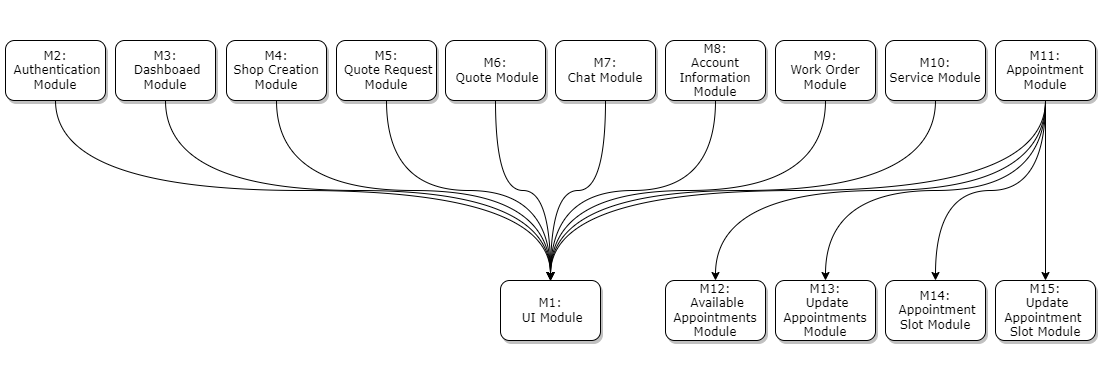
\includegraphics[width=1\textwidth]{UsesHierarchy.png}
\caption{Use hierarchy among modules}
\label{FigUH}
\end{figure}

%\section*{References}

\bibliographystyle {plainnat}
\bibliography{../../../refs/References}

\newpage{}
\end{document}